\documentclass{pennThesis}


%\title{Some ditau physics at atlas: a measurement of the \mbox{$Z\rightarrow\tau\tau$} cross section, and a search for high-mass resonances decaying to $\tau^{+}\tau^{-}$ in the atlas detector}
%\title{a search for new physics in high-mass ditau events in the atlas detector}
\title{a search for new physics in high-mass ditau events at atlas}
    
\author{Ryan Reece}

\newcommand{\adviser}{H.H. Williams, Professor, Physics}
\newcommand{\advisershort}{H.H. Williams}

\newcommand{\myinstitution}{The Univeristy of Pennsylvania}

\newcommand{\chairperson}{A.T. Charlie Johnson, Professor, Physics}

%\newcommand{\committeeOne}{Gary Bernstein, Professor, Physics}
\newcommand{\committeeOne}{Randall Kamien, Professor, Physics}
%\newcommand{\committeeOne}{I. Joseph Kroll, Professor, Physics}
\newcommand{\committeeTwo}{I. Joseph Kroll, Professor, Physics}
%\newcommand{\committeeTwo}{Elliot Lipeles, Assistant Professor, Physics}
\newcommand{\committeeThree}{Elliot Lipeles, Assistant Professor, Physics}
%\newcommand{\committeeThree}{Burt Ovrut, Professor, Physics}
\newcommand{\committeeFour}{Burt Ovrut, Professor, Physics}
%\newcommand{\committeeFour}{Masao Sako, Assistant Professor, Physics}
%\newcommand{\committeeFour}{Evelyn Thomson, Associate Professor, Physics}

\draftversion{00-01}

\newboolean{springer}
\setboolean{springer}{false}


\usepackage{atlasphysics}
\usepackage{thesisstyle}

%% feynmf for feynman diagrams
\usepackage{xspace}
\usepackage{feynmf}
\usepackage{threeparttable}
\setlength{\unitlength}{1mm}

%% other std packages
\usepackage{multirow}
%\usepackage{subfig}


\begin{document}
\begin{fmffile}{thesis-feyn}

%%--------------------------------------------------------------------
%% title page
%% copyright
%% acknowledgements
%% abstract
%%--------------------------------------------------------------------
\frontmatter
\maketitle

%%--------------------------------------------------------------------
%% table of contents
%% list of tables
%% list of figures
%%--------------------------------------------------------------------
\begin{Spacing}{\mylinespacing}
\tableofcontents
\end{Spacing}
\clearpage

%% let the list of tables and figures use the default single-spacing
 \makeatletter
    \renewcommand*\l@figure{\@dottedtocline{1}{1em}{3.2em}}
 \makeatother
 \listoftables
 \clearpage
 \listoffigures
 \clearpage

%%--------------------------------------------------------------------
%% preface
%%--------------------------------------------------------------------
\begin{Spacing}{\mylinespacing}
%
\chapter*{Preface}
\addcontentsline{toc}{chapter}{Preface}

This is the preface.

\vspace{0.05\textheight}

\begin{tabular}{p{0.5\textwidth} l}
  & Alexander Tuna   \\
  & CERN, March 2015 \\
\end{tabular}



%%--------------------------------------------------------------------
%% main sections
%%--------------------------------------------------------------------
\mainmatter

\chapter[Introduction][Introduction]{Introduction}
\chapter[Introduction][Introduction]{Introduction}
\label{chap:introduction}

This thesis documents the evidence of Higgs boson decays to tau leptons with the ATLAS detector at the LHC. Special focus is given to the $\taul\tauh$ subset of the analysis.

\cref{chap:standardmodel} gives a description of the Standard Model of particle physics to provide theoretical motivation for searches for the Higgs boson. \cref{chap:lhcatlas} describes the LHC and the ATLAS detector, which are the experimental apparatuses used here. \cref{chap:taus} describes tau leptons and their experimental signatures at ATLAS.

\cref{chap:strategy} describes the strategy for searching for $\Htautau$ at ATLAS. \cref{chap:backgrounds} reviews how physics processes relevant to the search are predicted, with special emphasis given to mis-identified $\tauh$. \cref{chap:results} gives the results of the searches. \cref{chap:prospects} concludes this with a discussion of future prospects for $\Htautau$ analysis at ATLAS, both in the near- and long-term.




\chapter[The Standard Model of particle physics][The Standard Model of particle physics]{The Standard Model of particle physics}
\include{theory}

\chapter[The LHC][The LHC]{The LHC}
\include{lhc}

\chapter[The ATLAS experiment][The ATLAS experiment]{The ATLAS experiment}
\include{atlas}

\chapter[Tau leptons at ATLAS][Tau leptons at ATLAS]{Tau leptons at ATLAS}
\chapter[Tau leptons][Tau leptons]{Tau leptons}
\label{chap:taus}

\begin{quote}
  Tau leptons and their signature in the ATLAS detector are described. 
\end{quote}

\section{Tau leptons}
\label{sec:taus-theory}

Tau leptons were discovered in the 1970s by Martin Perl and the SLAC-LBL group at the SPEAR electron-positron collider~\cite{1975.Perl.discovery_of_tau_1,1976.Perl.discovery_of_tau_2,1977.Perl.discovery_of_tau_3}. They have since been studied in great detail at experiments like Belle and BaBar. The associated tau neutrino was first observed directly at the DONUT experiment in 2000, though its existence was inferred by measurements of the width of the $Z$ boson by experiments at the LEP collider in 1990.

Tau leptons are the heaviest of the charged leptons. Their mass of 1.78 GeV is approximately twenty times larger than the muon mass, and their short lifetime $c\tau = \text{87} \mu m$ implies tau leptons produced in $pp$ collisions at the LHC typically decay within the ATLAS beam pipe. The ATLAS detector therefore observes only the decay products of the tau lepton, not the particle itself.

Tau leptons decay leptonically in 35\% of decays and hadronically in 65\%. Among hadronic decays, 72\% involve exactly one charged pion and 22\% exactly three charged pions. The remaining percentage of hadronic decays dominantly involves kaons or five (or more) charged pions. All tau lepton decays involve at least one neutrino. A pie chart of tau lepton branching fraction is given in \cref{fig:taus-decaypie}.


\begin{figure}[tp]
  \centering
  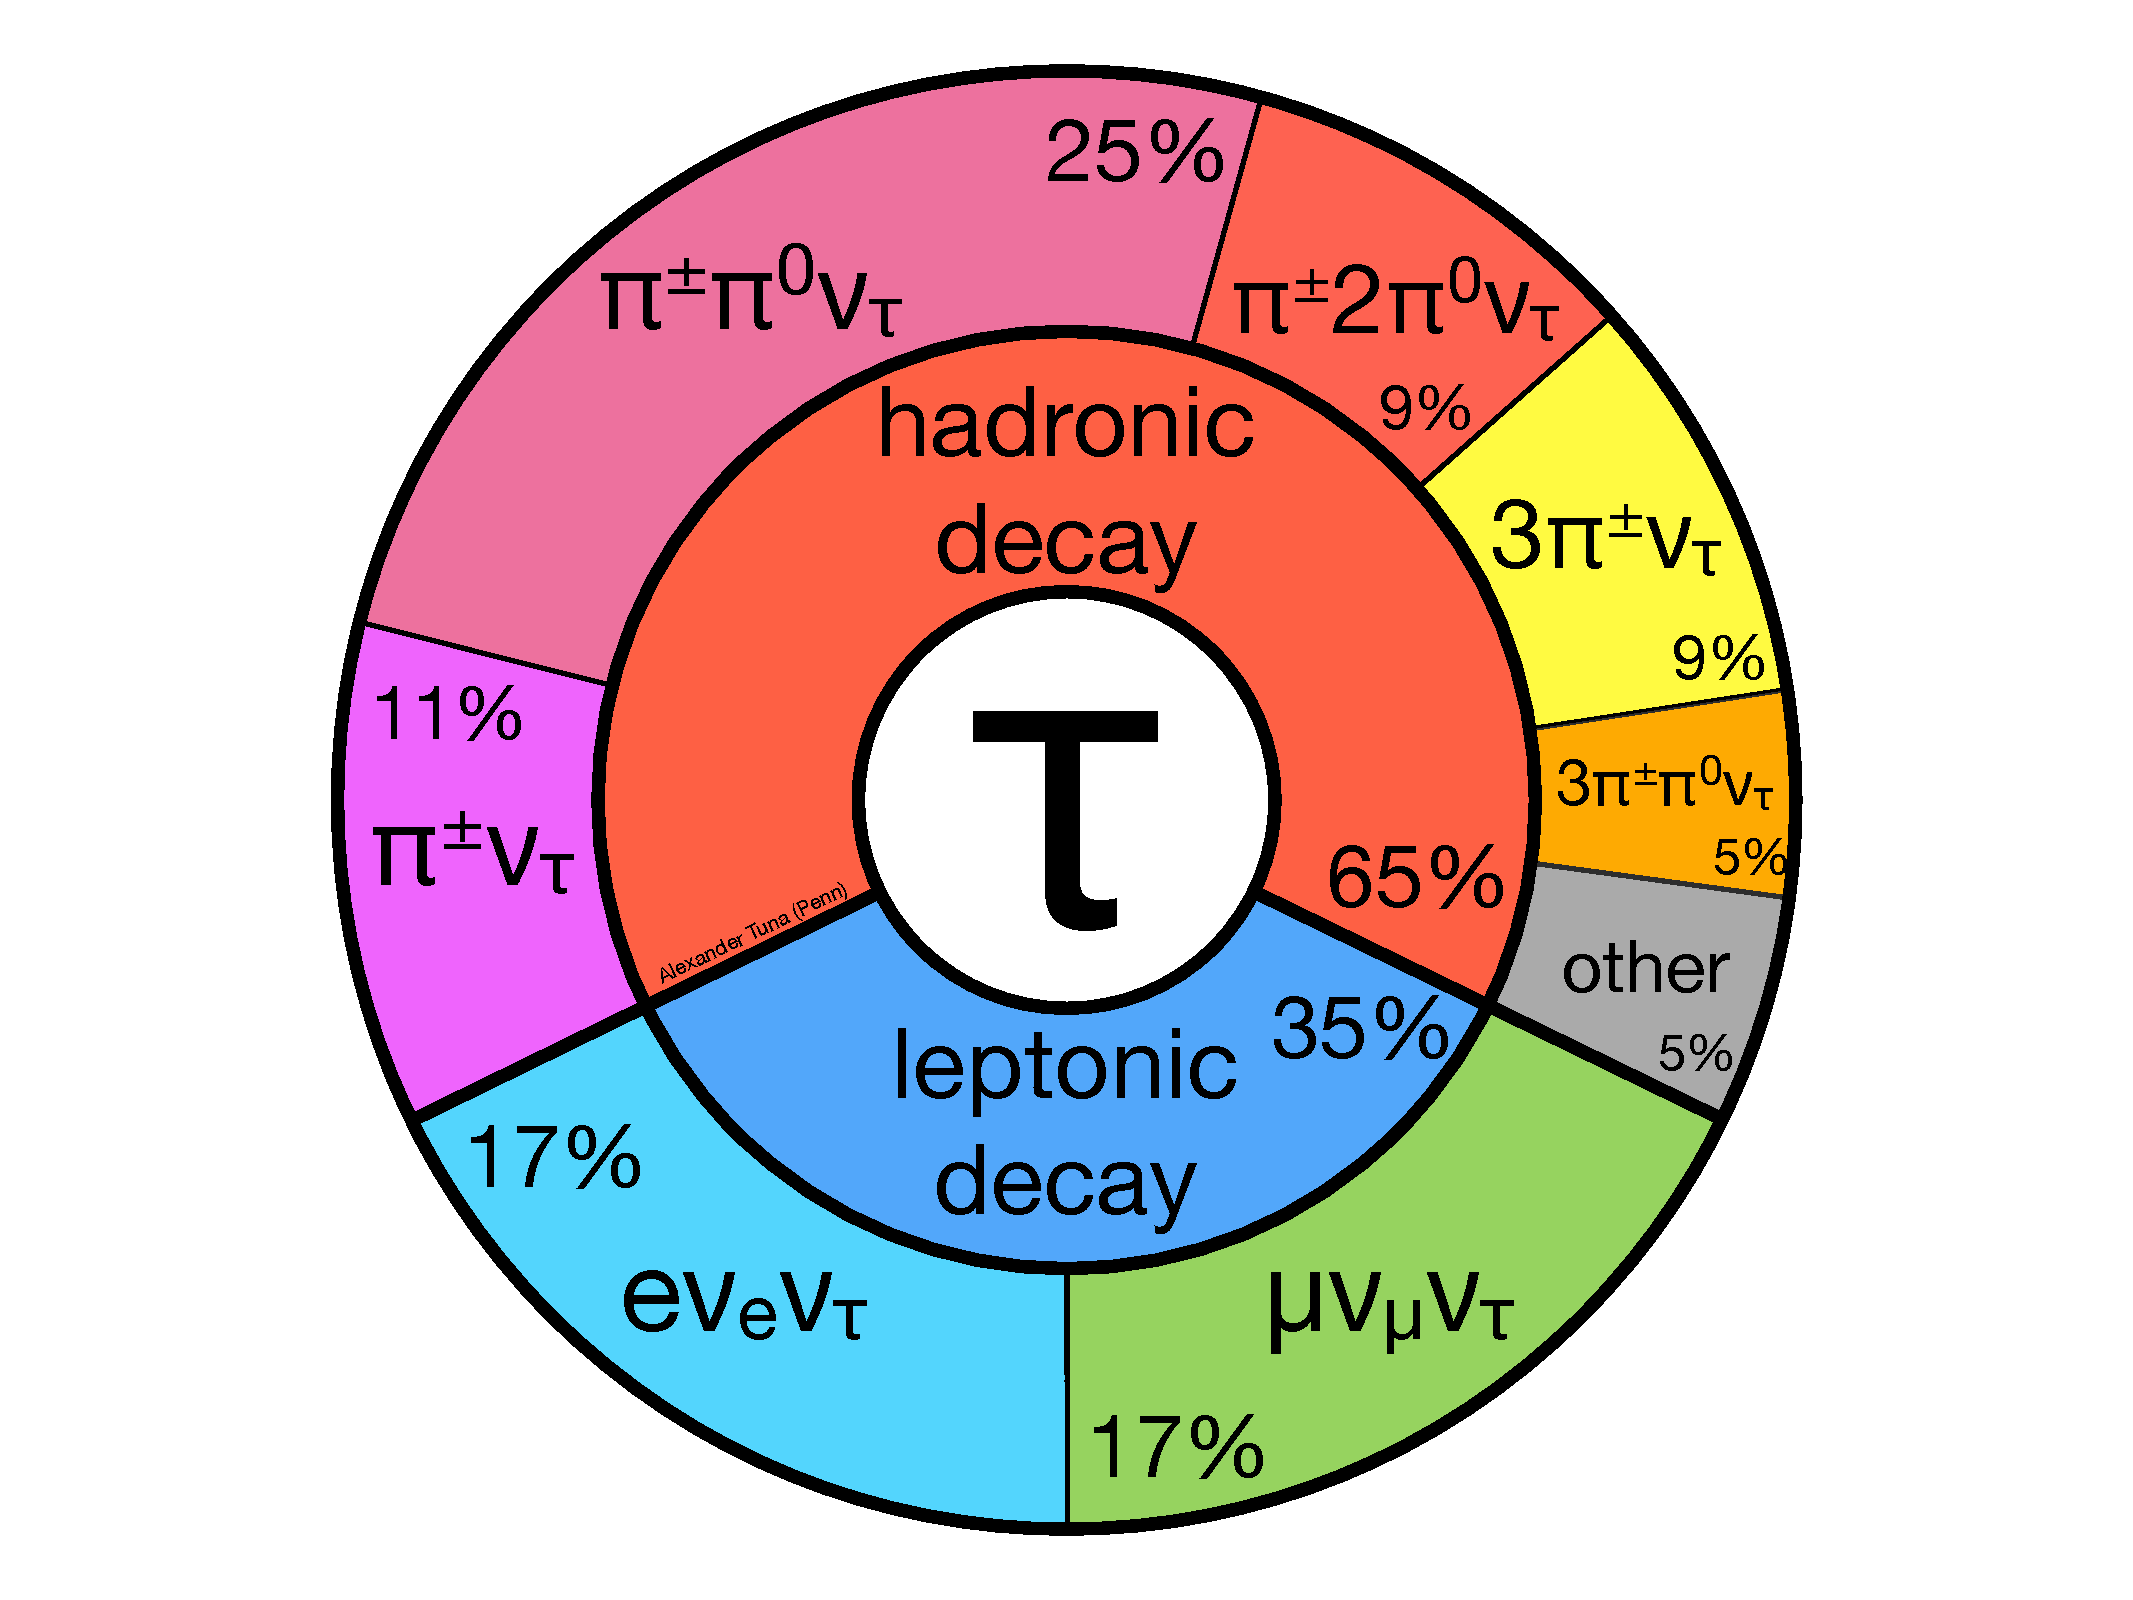
\includegraphics[width=0.48\textwidth]{figures/piecharts/taudecay}
  \caption{Variables.}
  \label{fig:taus-decaypie}
\end{figure}

\section{Leptonic tau decays, $\taul$}
\label{sec:taus-leptons}

\begin{figure}[tp]
  \centering
  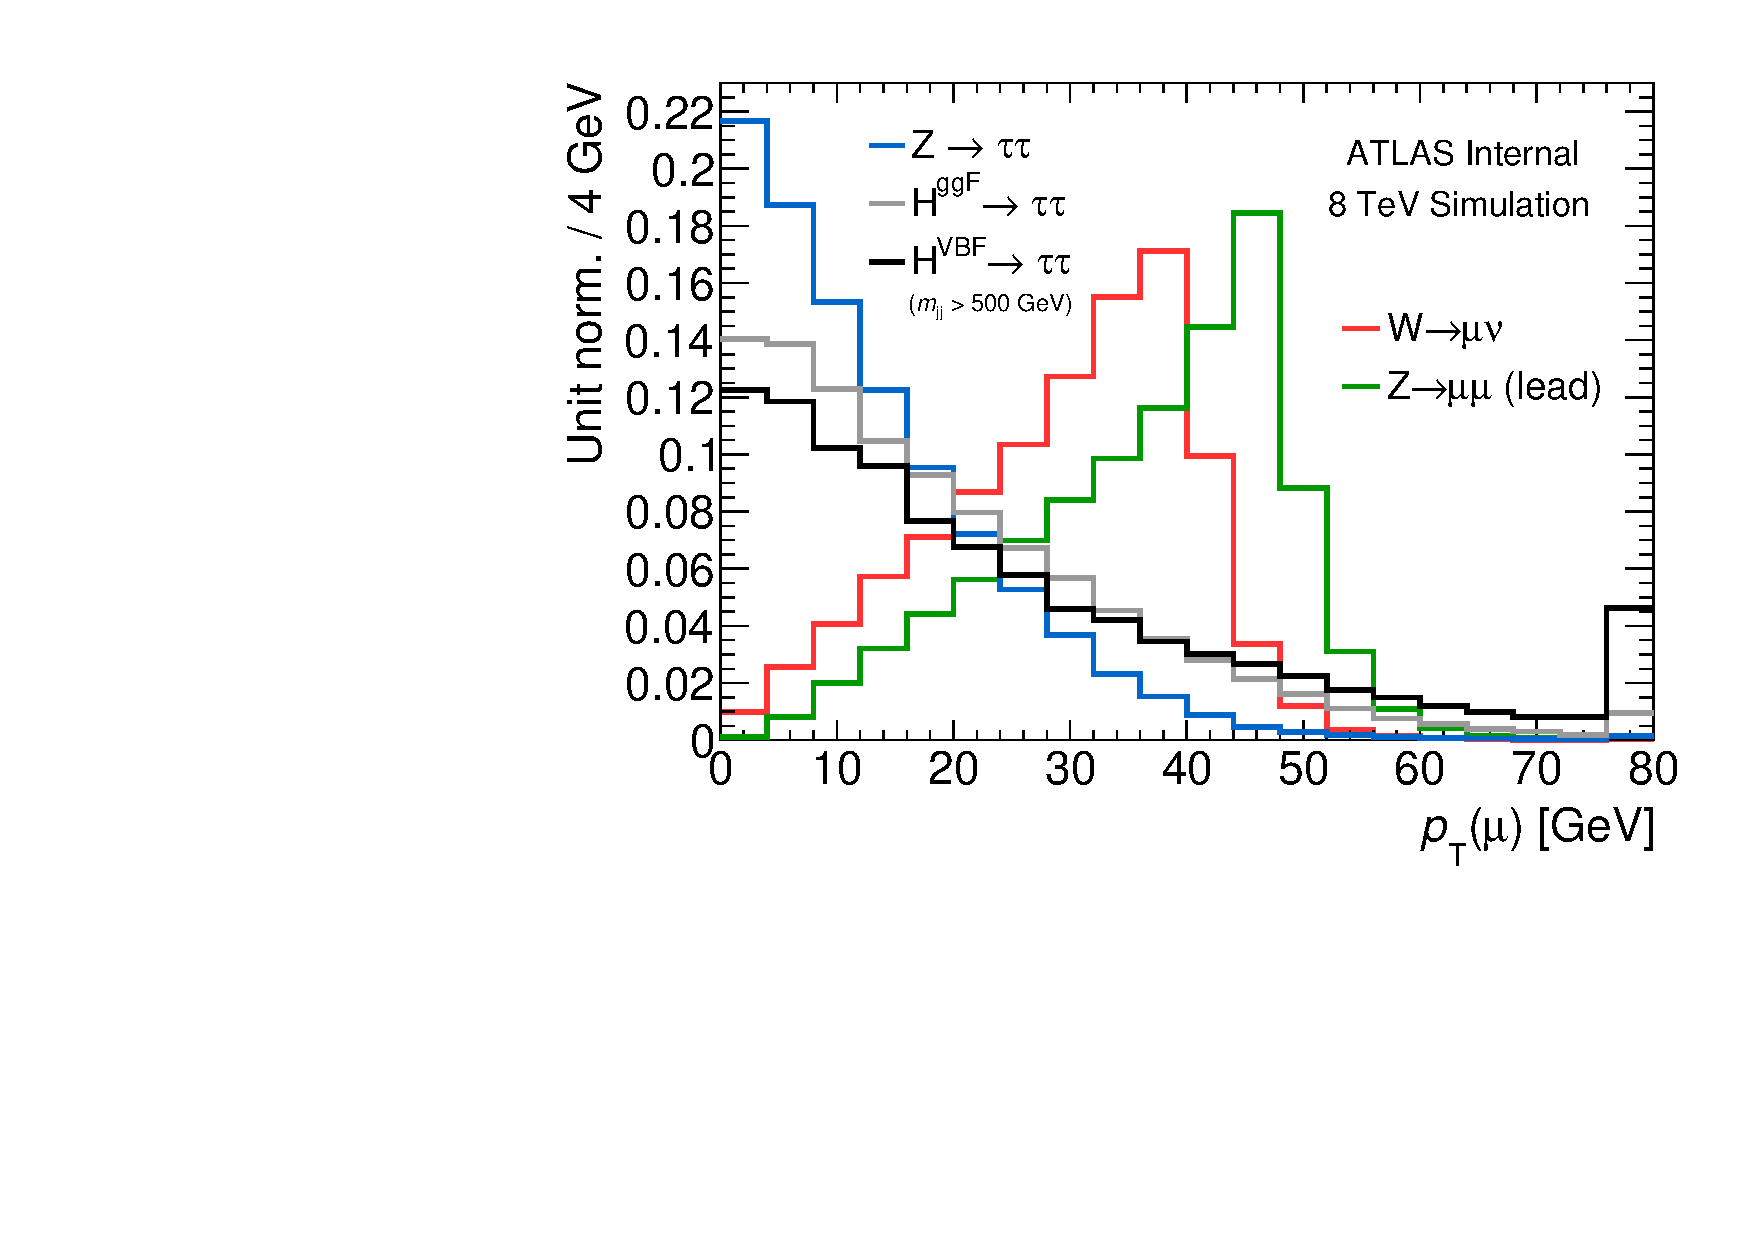
\includegraphics[width=0.7\textwidth]{figures/tauperformance/leptonsfromtausaresoft}
  \caption{Variables.}
  \label{fig:taus-leptonpt}
\end{figure}

\section{Hadronic tau decays, $\tauh$}
\label{sec:taus-jetfakes}

\begin{figure}[tp]
  \centering
  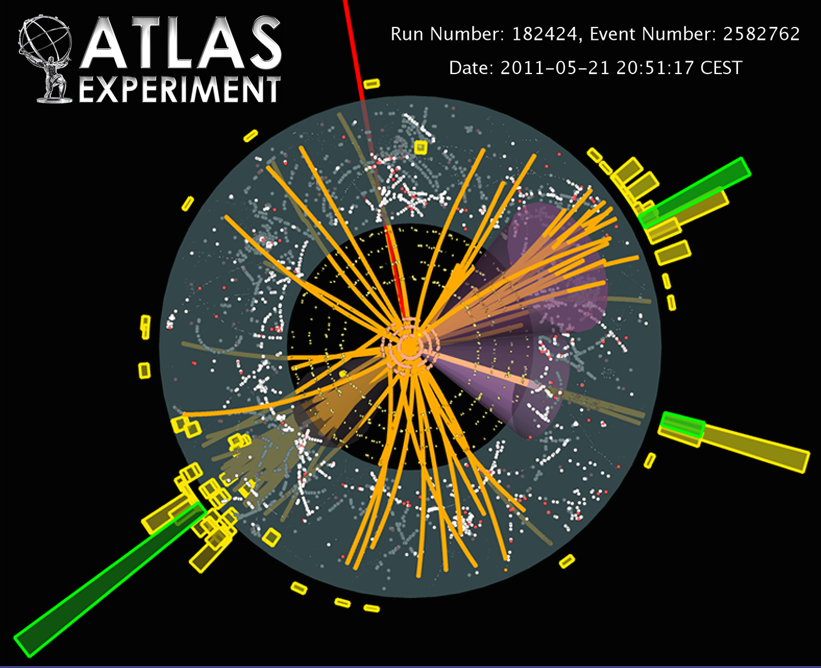
\includegraphics[width=0.95\textwidth]{figures/tauperformance/vp1_3dcocktail_run182424_evt2582762_tttaumu}
  \caption{Variables.}
  \label{fig:taus-eventdisplay}
\end{figure}

\begin{figure}[tp]
  \centering
  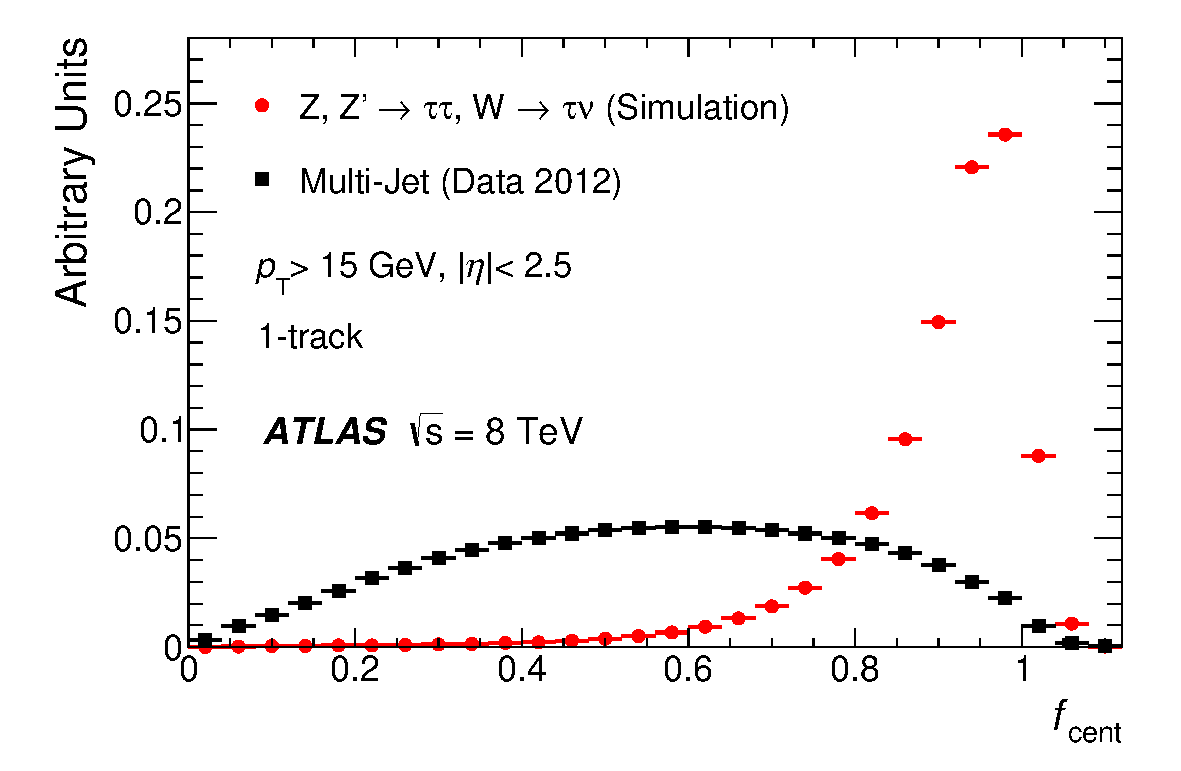
\includegraphics[width=0.48\textwidth]{figures/PERF-2013-06/fig_02a}
  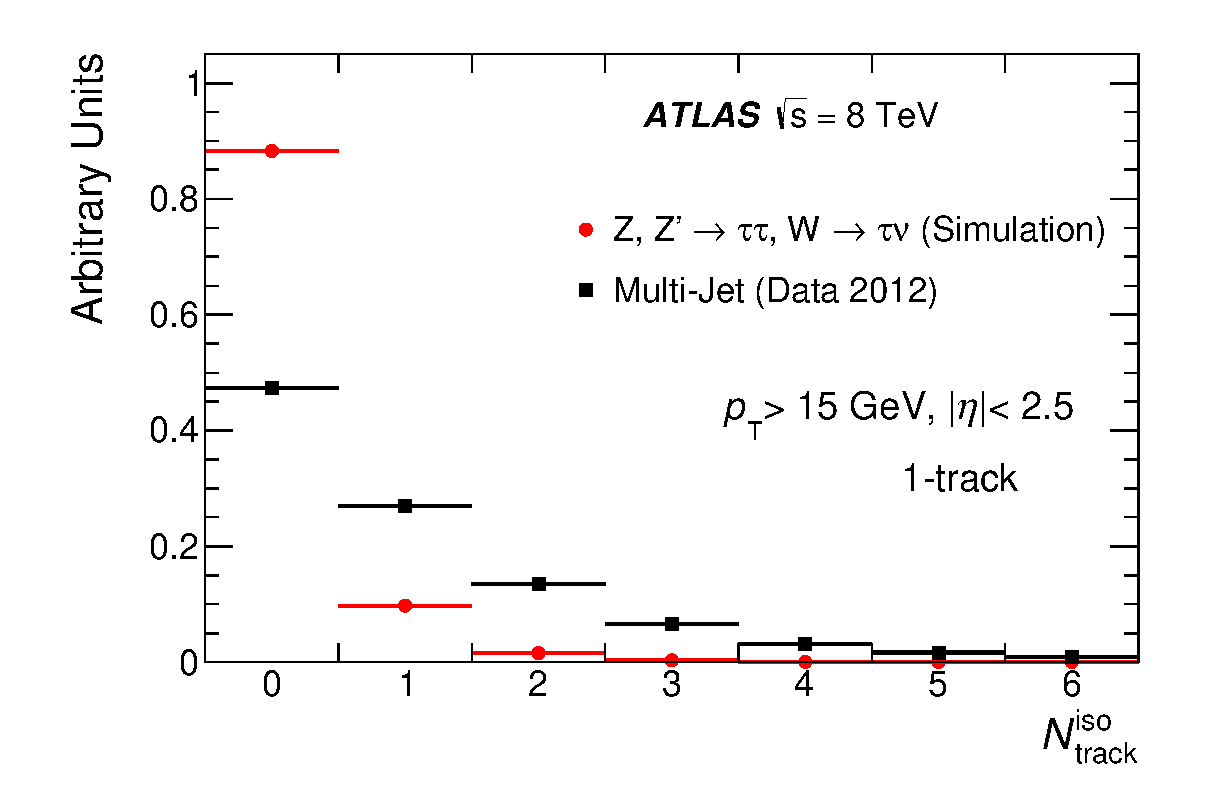
\includegraphics[width=0.48\textwidth]{figures/PERF-2013-06/fig_02b}
  \caption{Variables.}
  \label{fig:taus-id1p}
\end{figure}

\begin{figure}[tp]
  \centering
  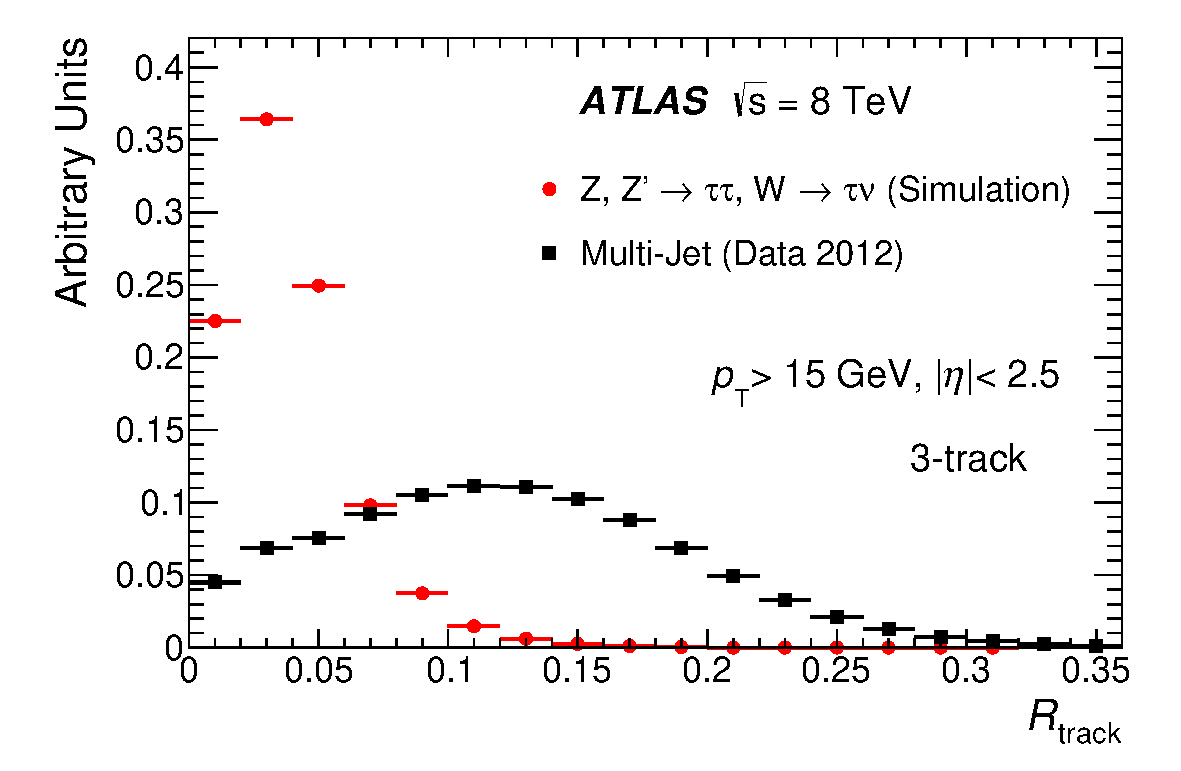
\includegraphics[width=0.48\textwidth]{figures/PERF-2013-06/fig_03a}
  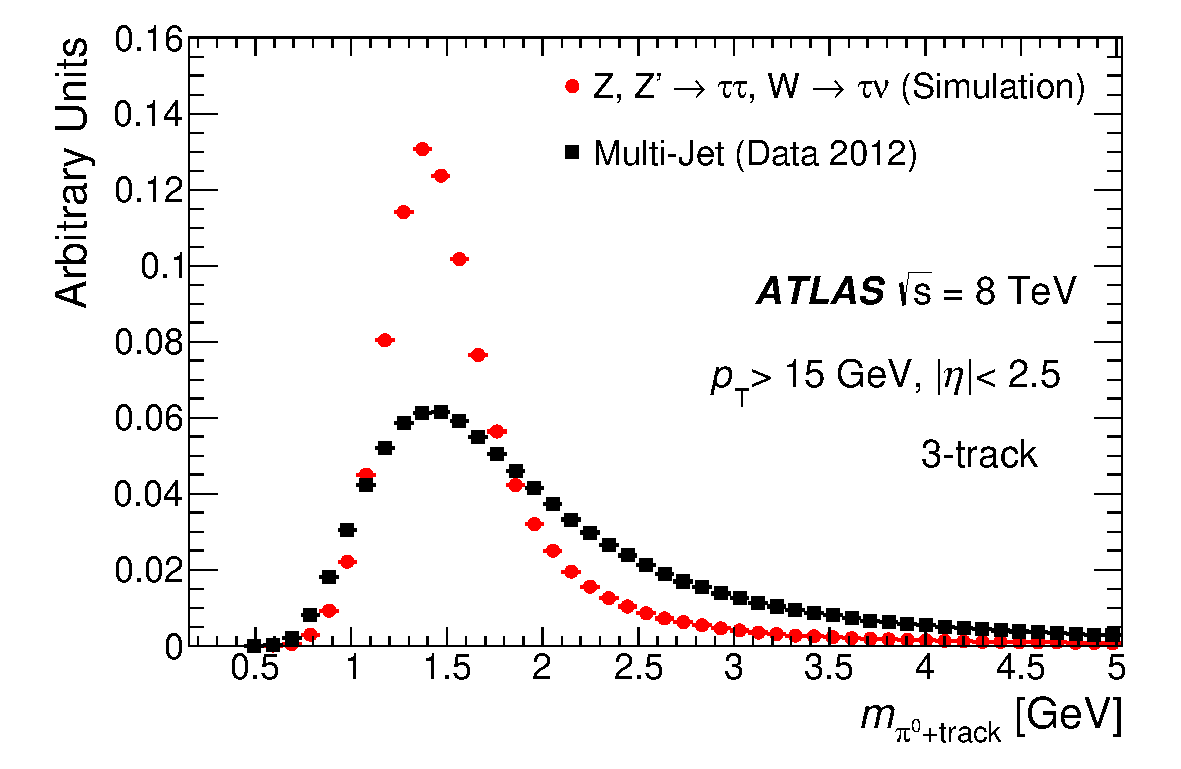
\includegraphics[width=0.48\textwidth]{figures/PERF-2013-06/fig_03b}
  \caption{Variables.}
  \label{fig:taus-id3p}
\end{figure}

\begin{figure}[tp]
  \centering
  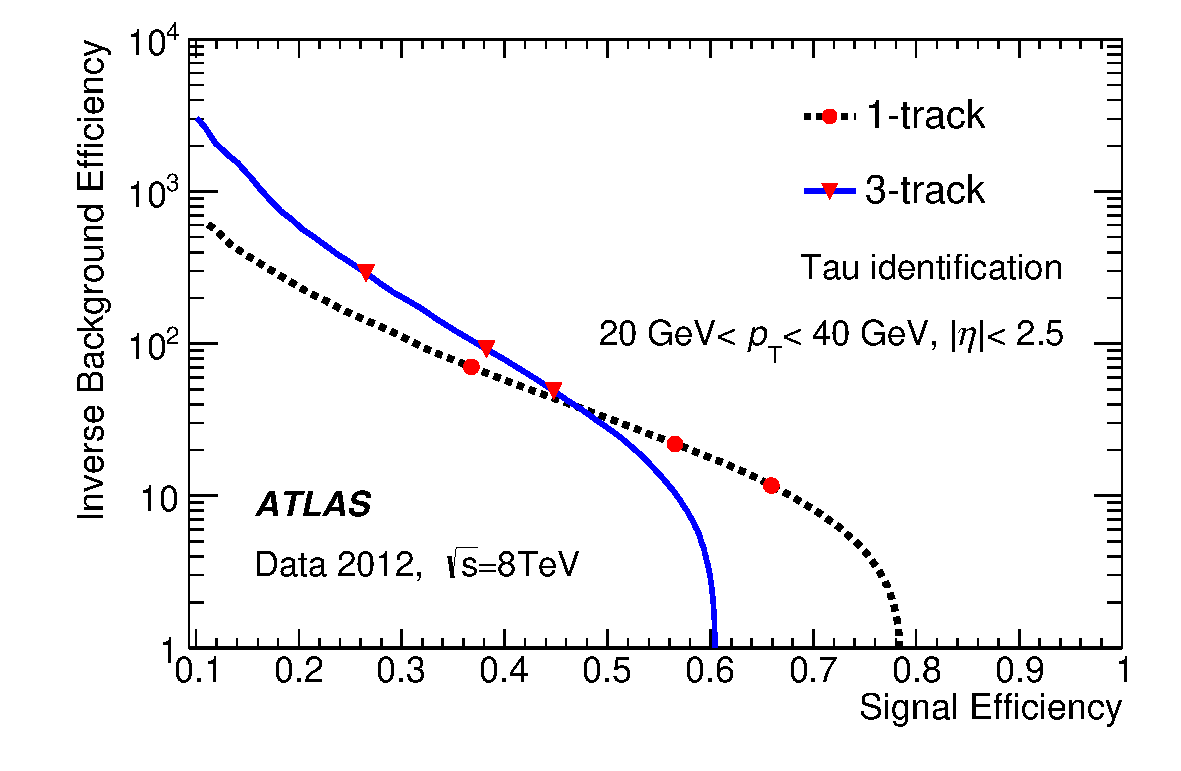
\includegraphics[width=0.48\textwidth]{figures/PERF-2013-06/fig_05a}
  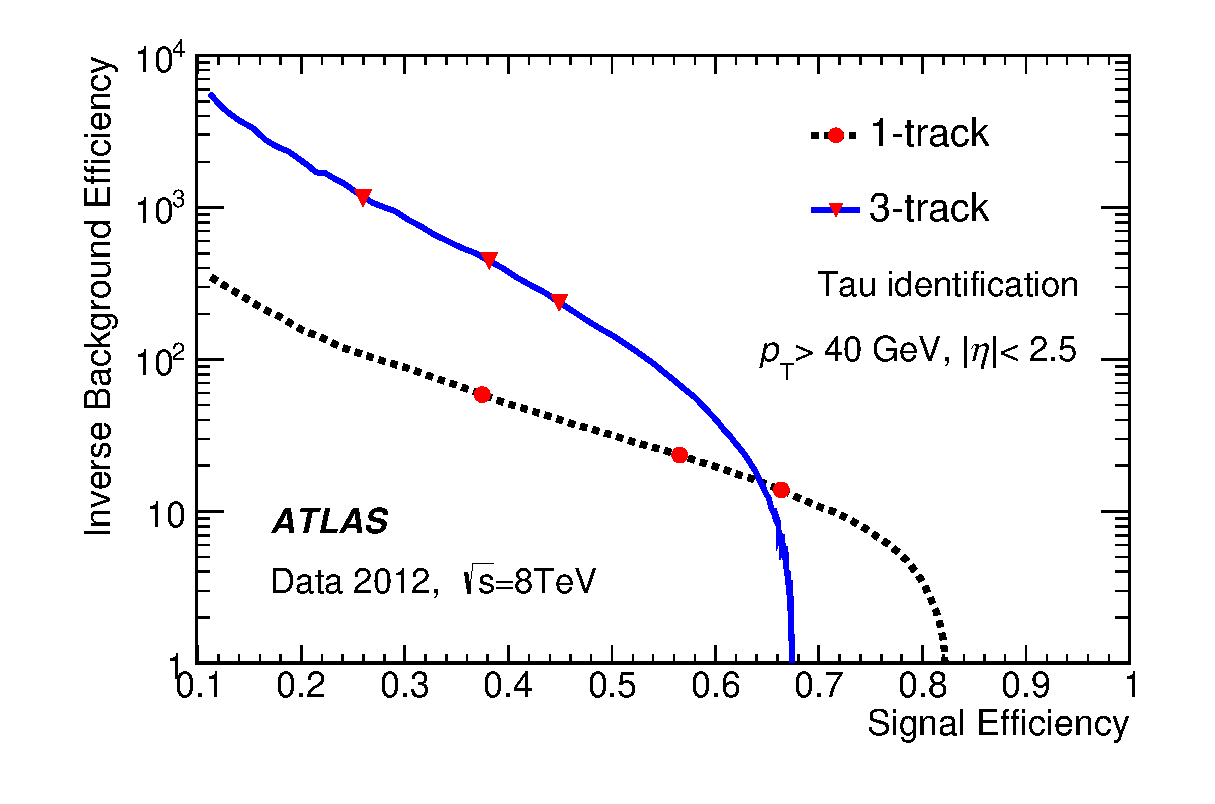
\includegraphics[width=0.48\textwidth]{figures/PERF-2013-06/fig_05b}
  \caption{Variables.}
  \label{fig:taus-idroc}
\end{figure}

\section{Leptons mis-identified as $\tauh$}
\label{sec:taus-leptonfakes}

\begin{figure}[tp]
  \centering
  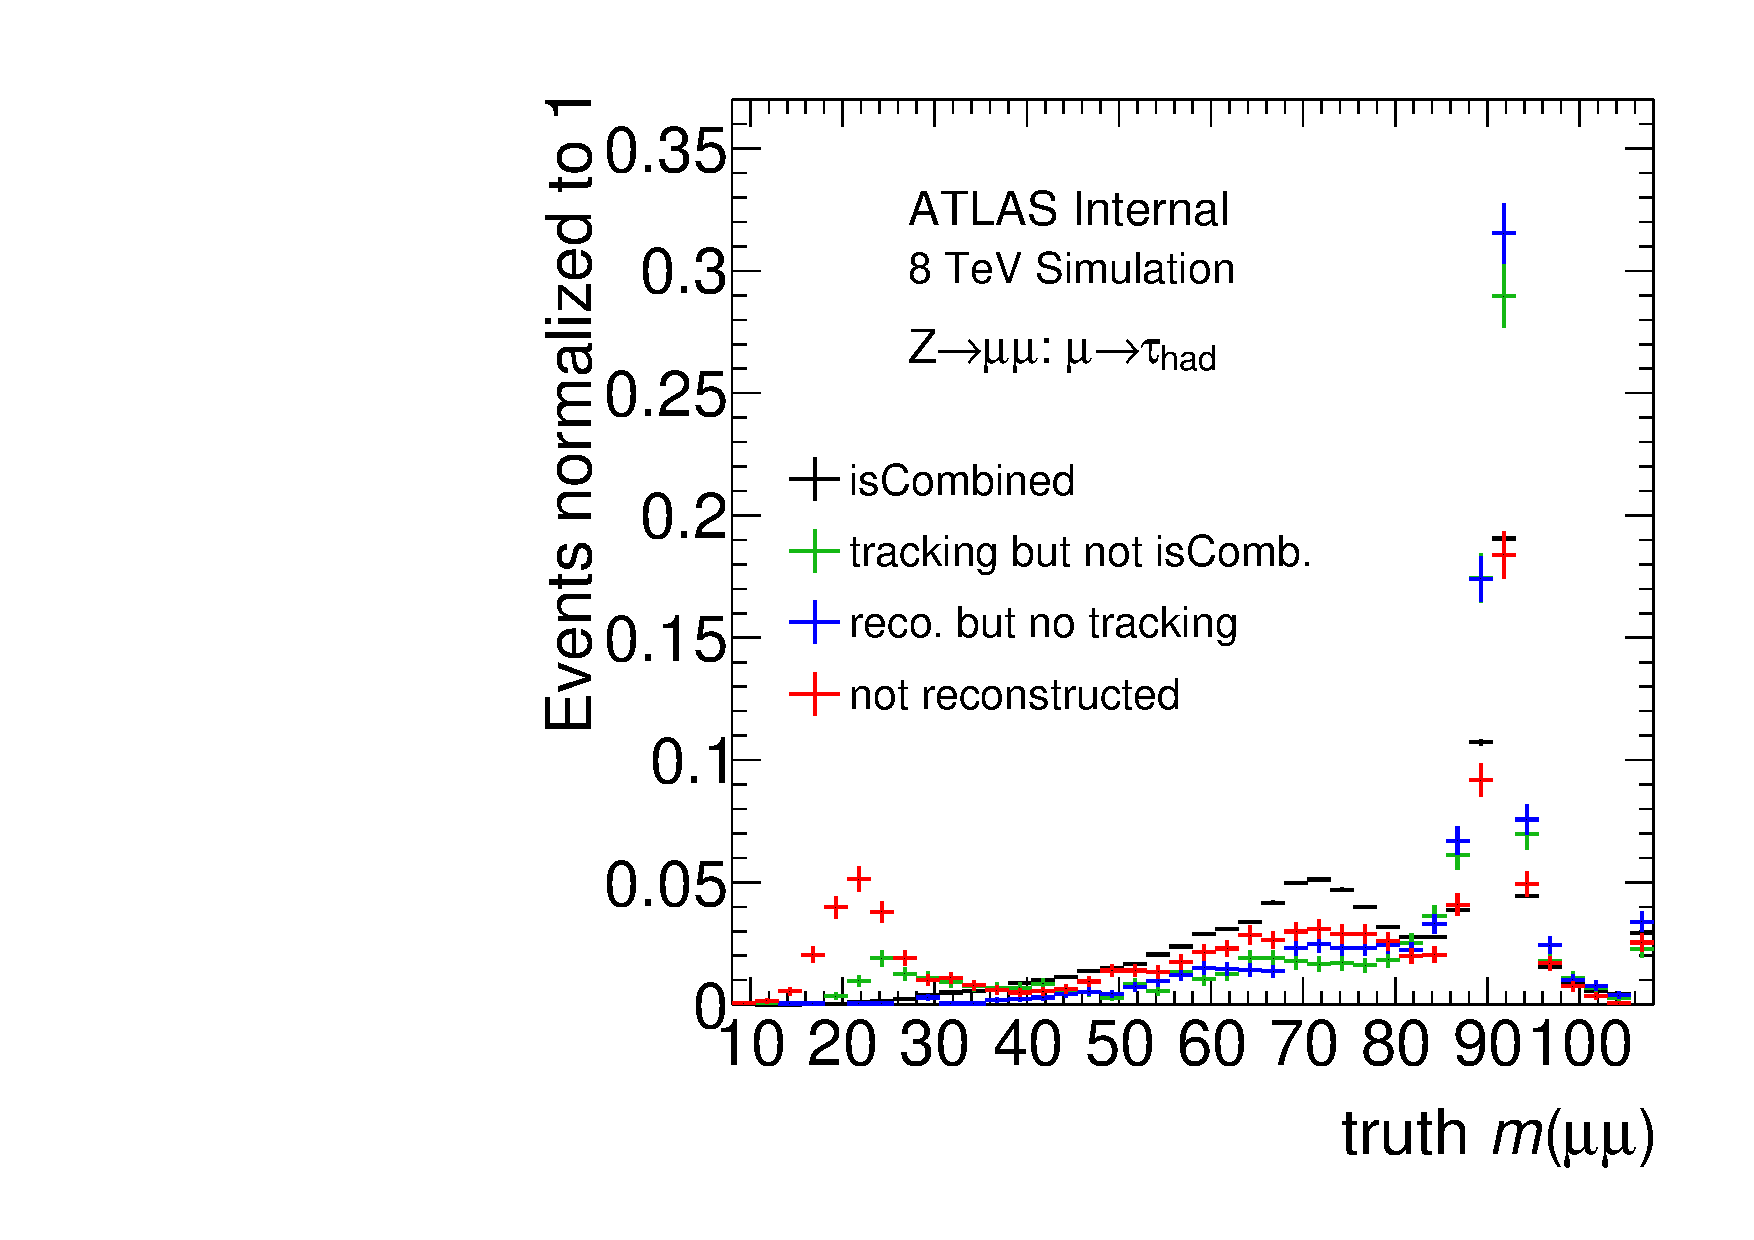
\includegraphics[width=0.48\textwidth]{figures/tauperformance/muonfakes_mll}
  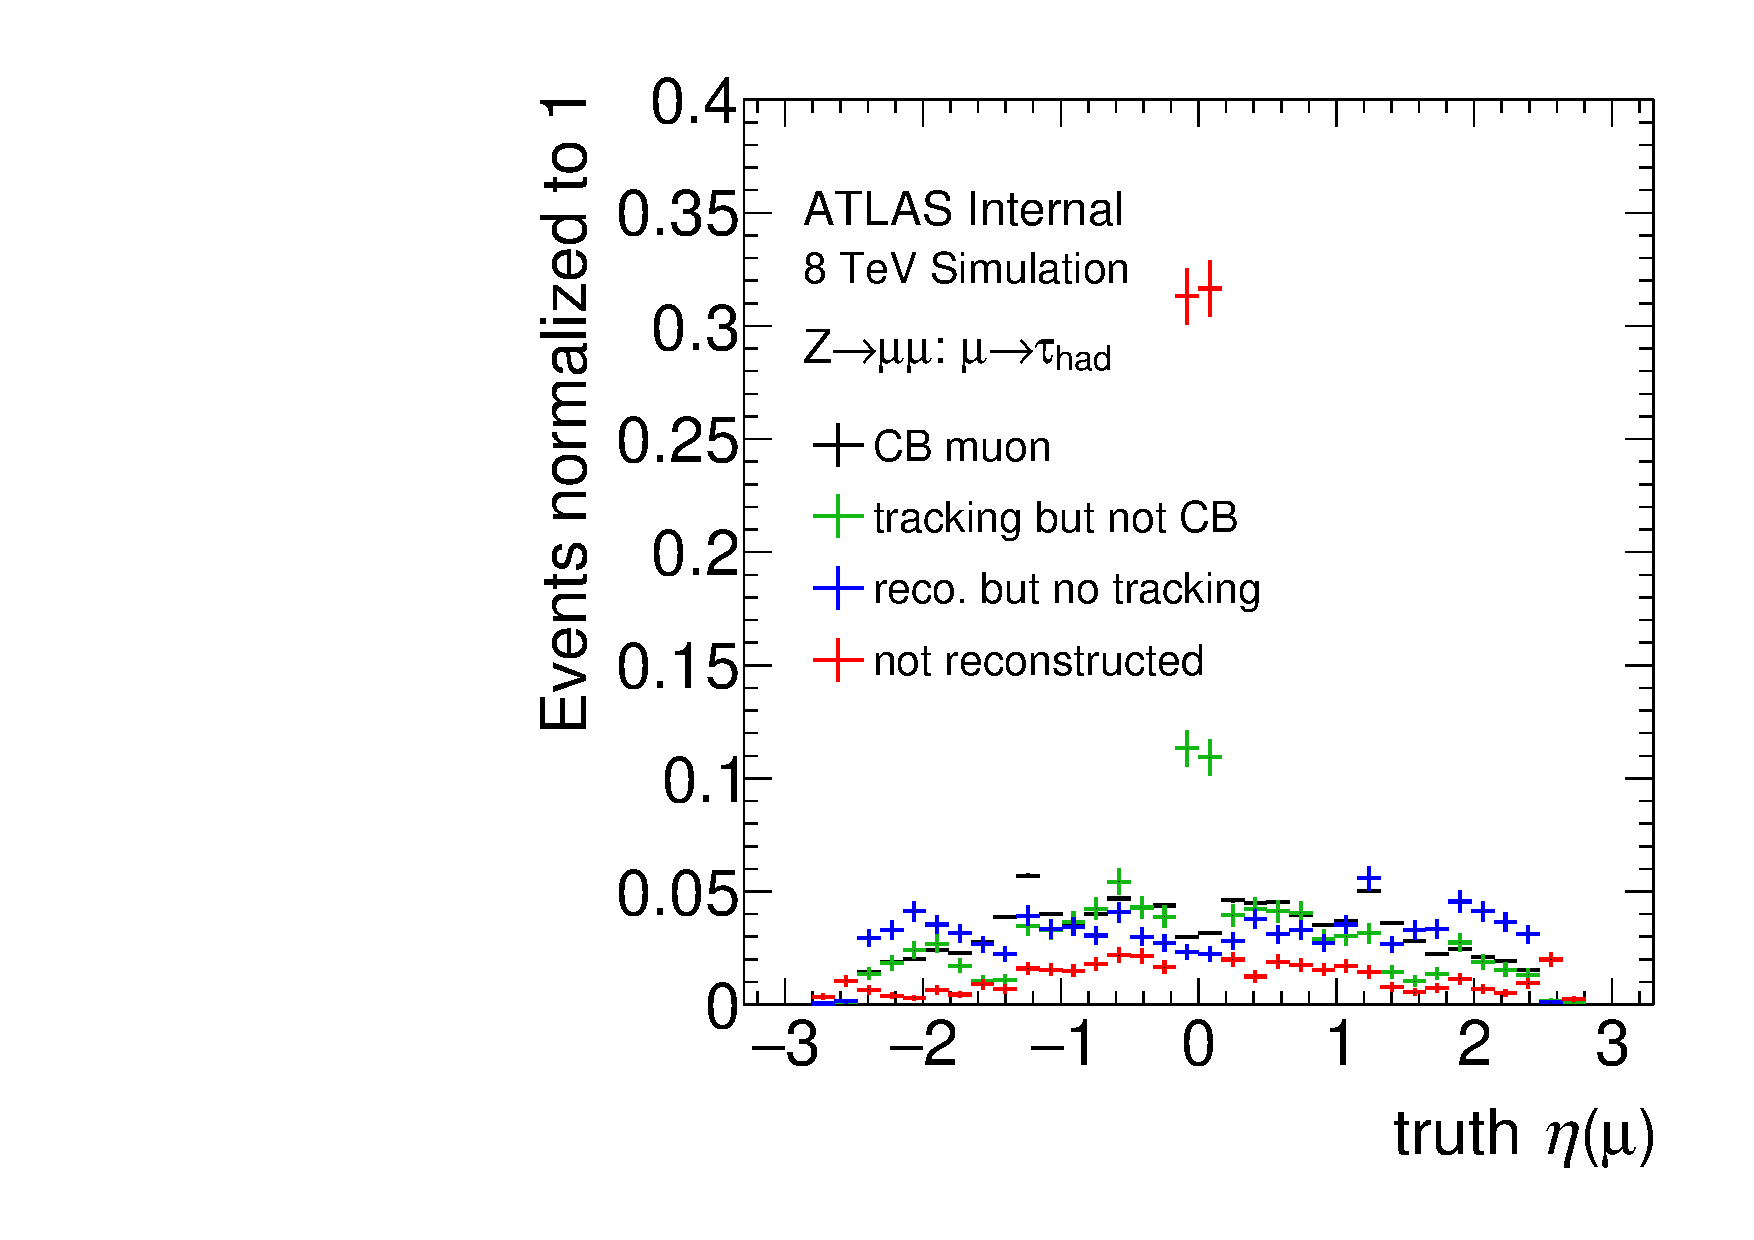
\includegraphics[width=0.48\textwidth]{figures/tauperformance/muonfakes_eta}
  \caption{Variables.}
  \label{fig:taus-muonfakes1}
\end{figure}

\begin{figure}[tp]
  \centering
  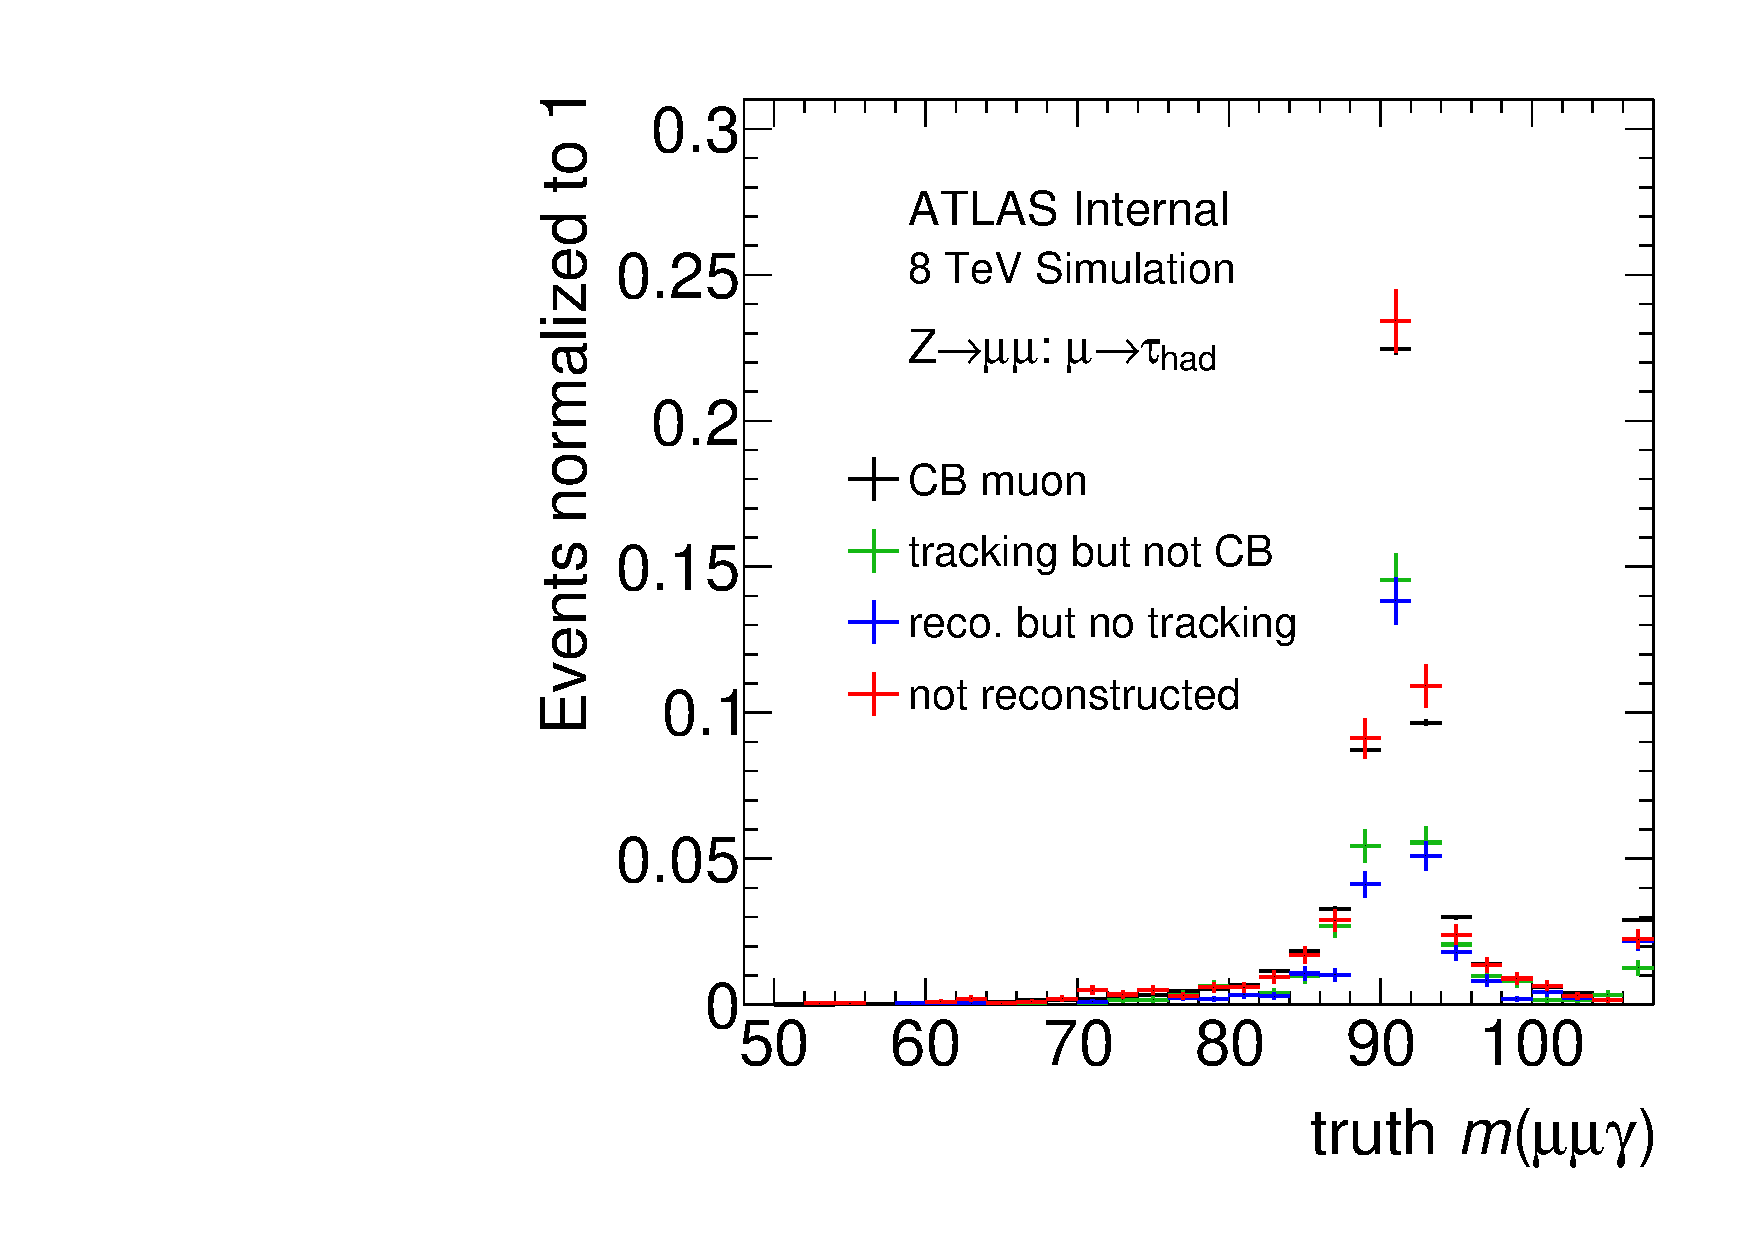
\includegraphics[width=0.48\textwidth]{figures/tauperformance/muonfakes_mlly}
  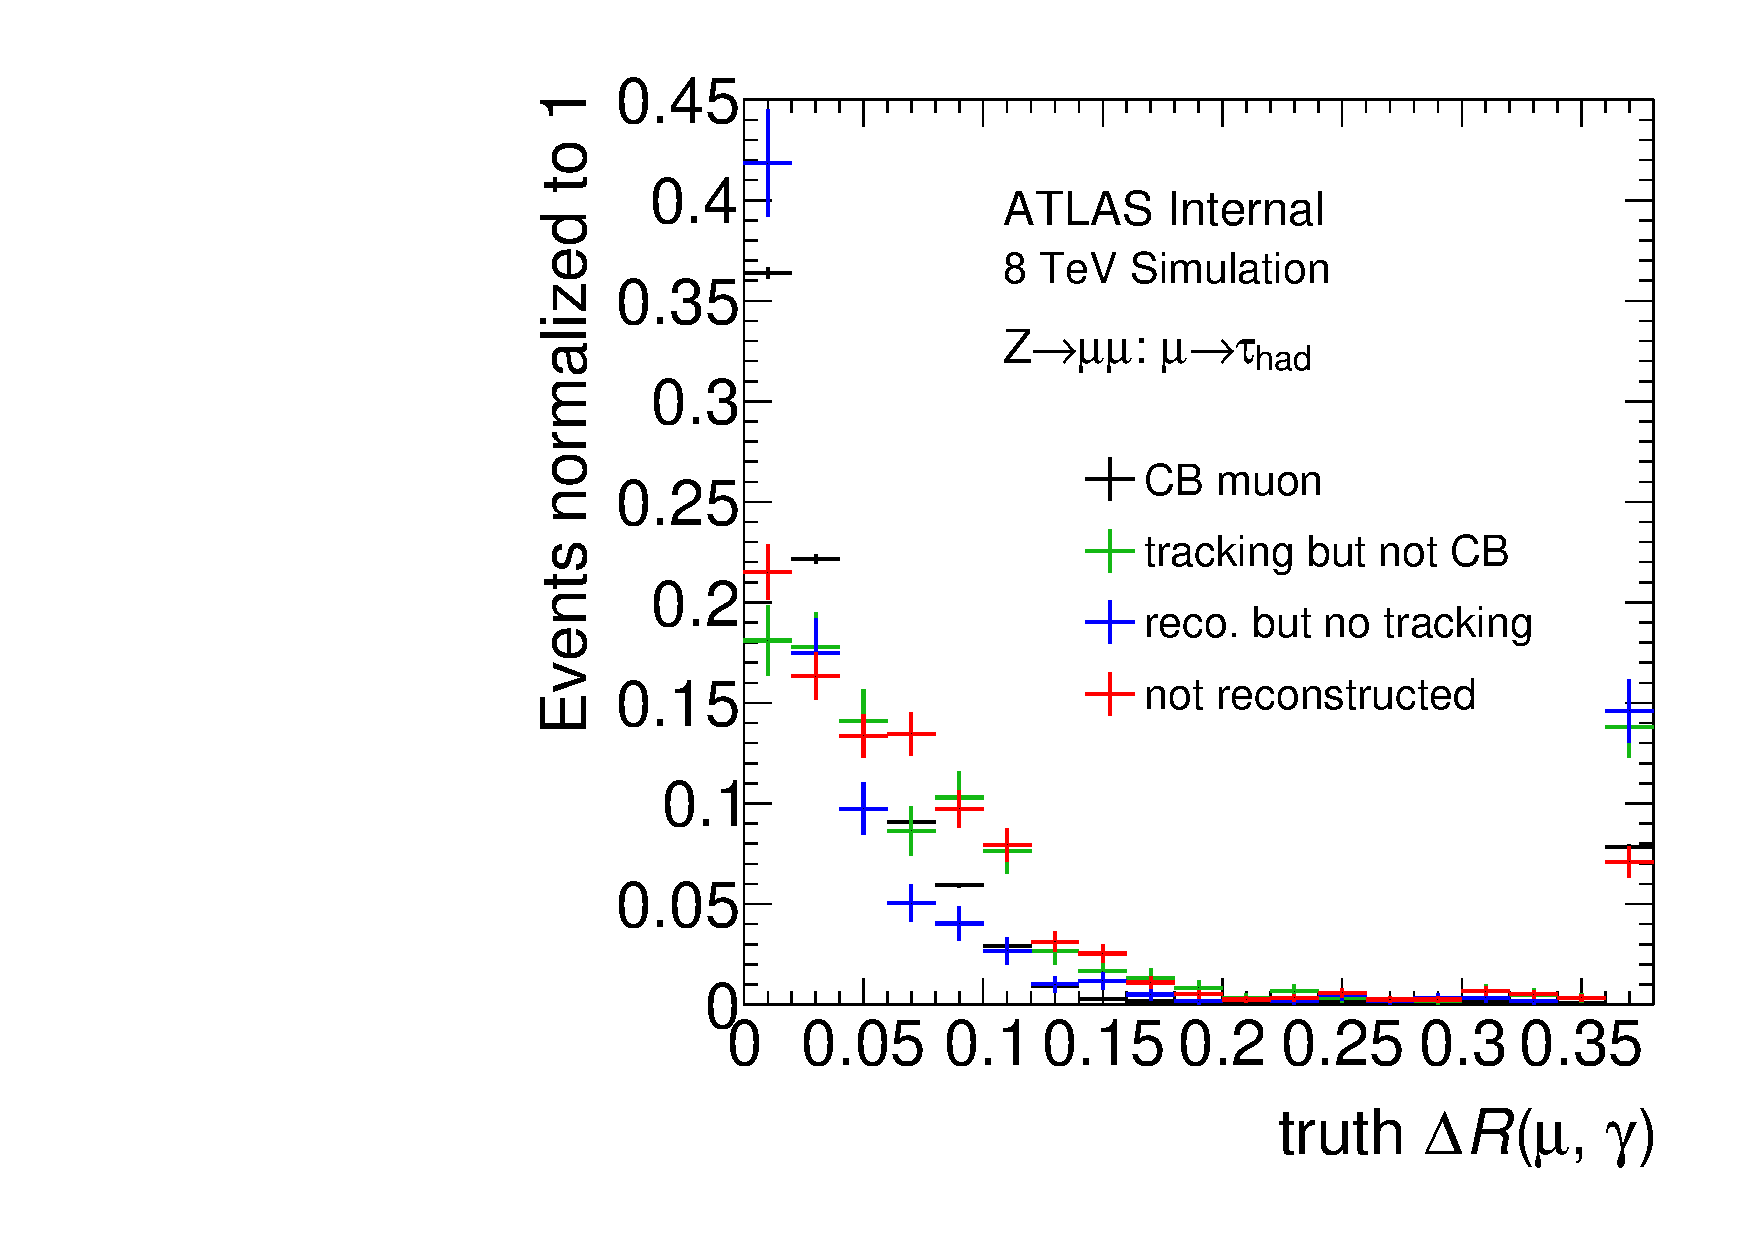
\includegraphics[width=0.48\textwidth]{figures/tauperformance/muonfakes_dR}
  \caption{Variables.}
  \label{fig:taus-muonfakes2}
\end{figure}

\begin{figure}[tp]
  \centering
  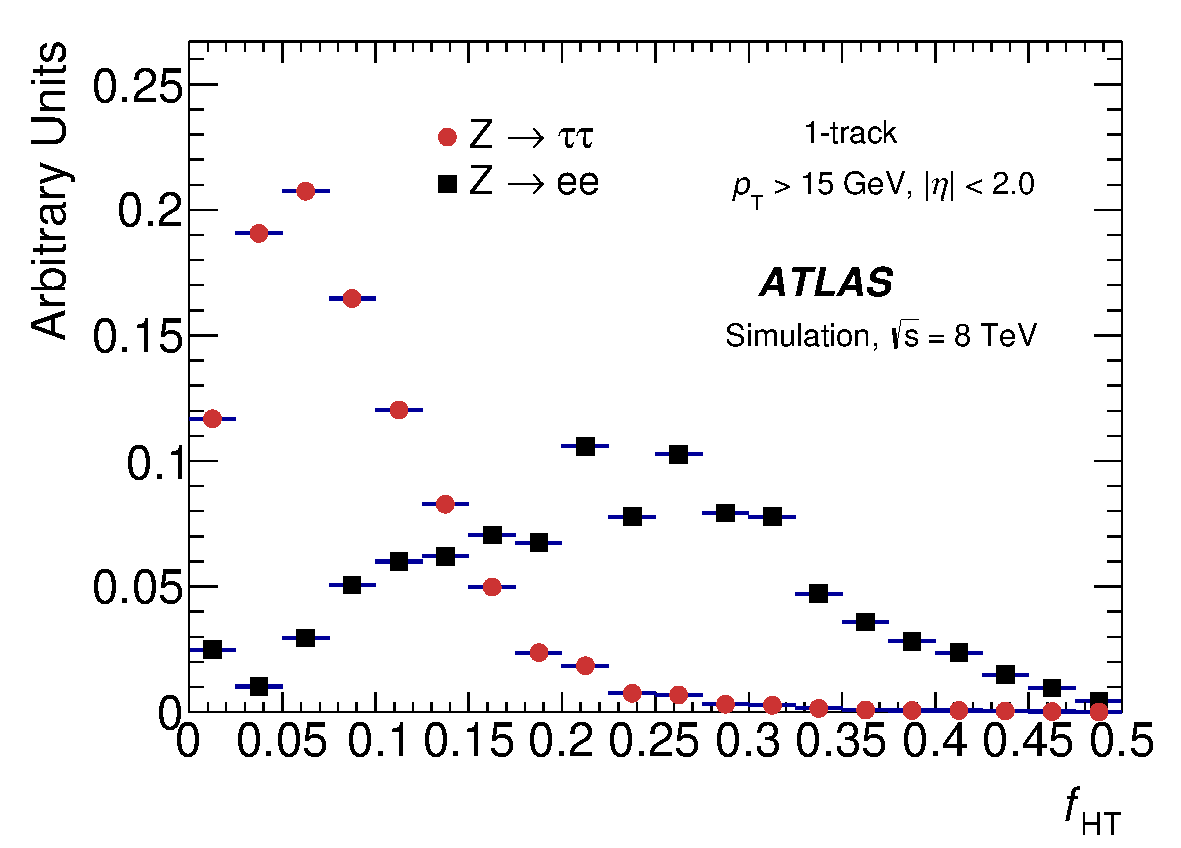
\includegraphics[width=0.48\textwidth]{figures/PERF-2013-06/fig_08a}
  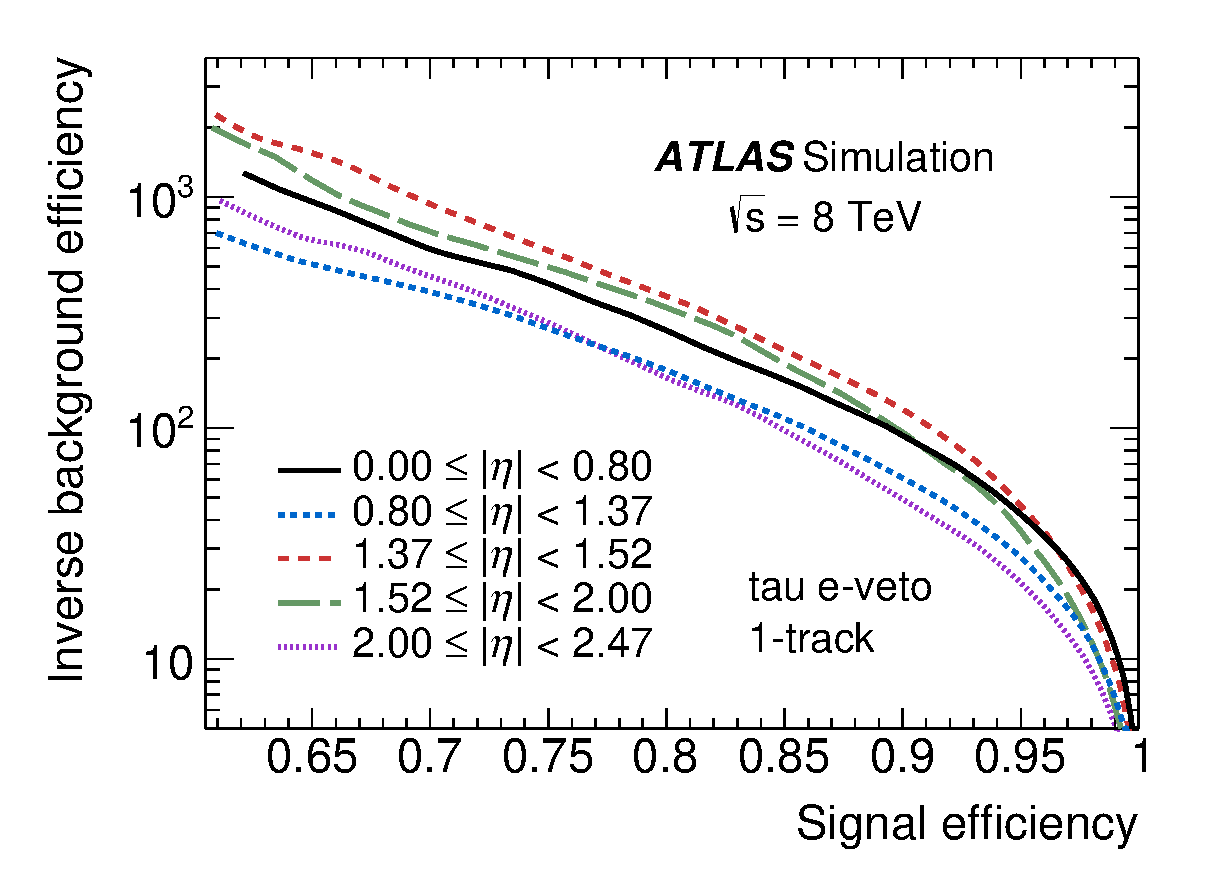
\includegraphics[width=0.48\textwidth]{figures/PERF-2013-06/fig_09}
  \caption{Variables.}
  \label{fig:taus-electronfakes1}
\end{figure}

\begin{figure}[tp]
  \centering
  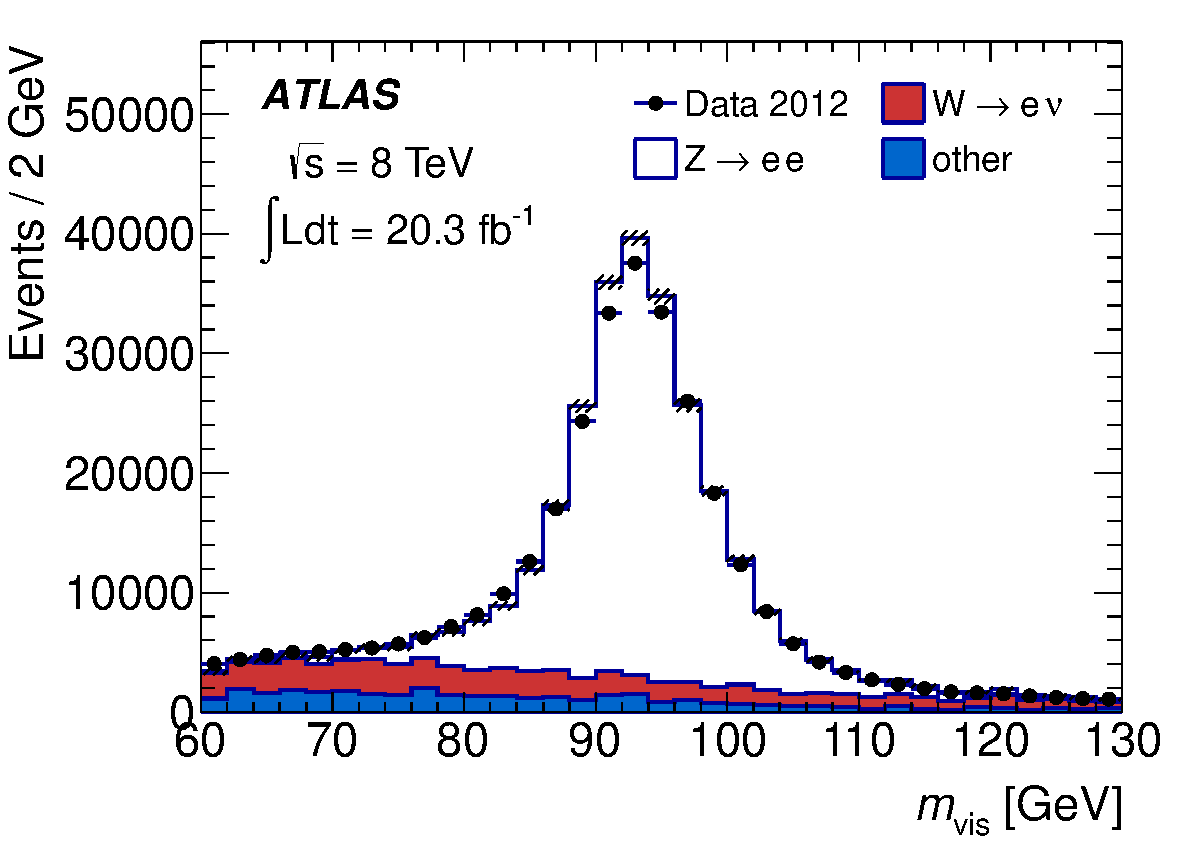
\includegraphics[width=0.48\textwidth]{figures/PERF-2013-06/fig_14a}
  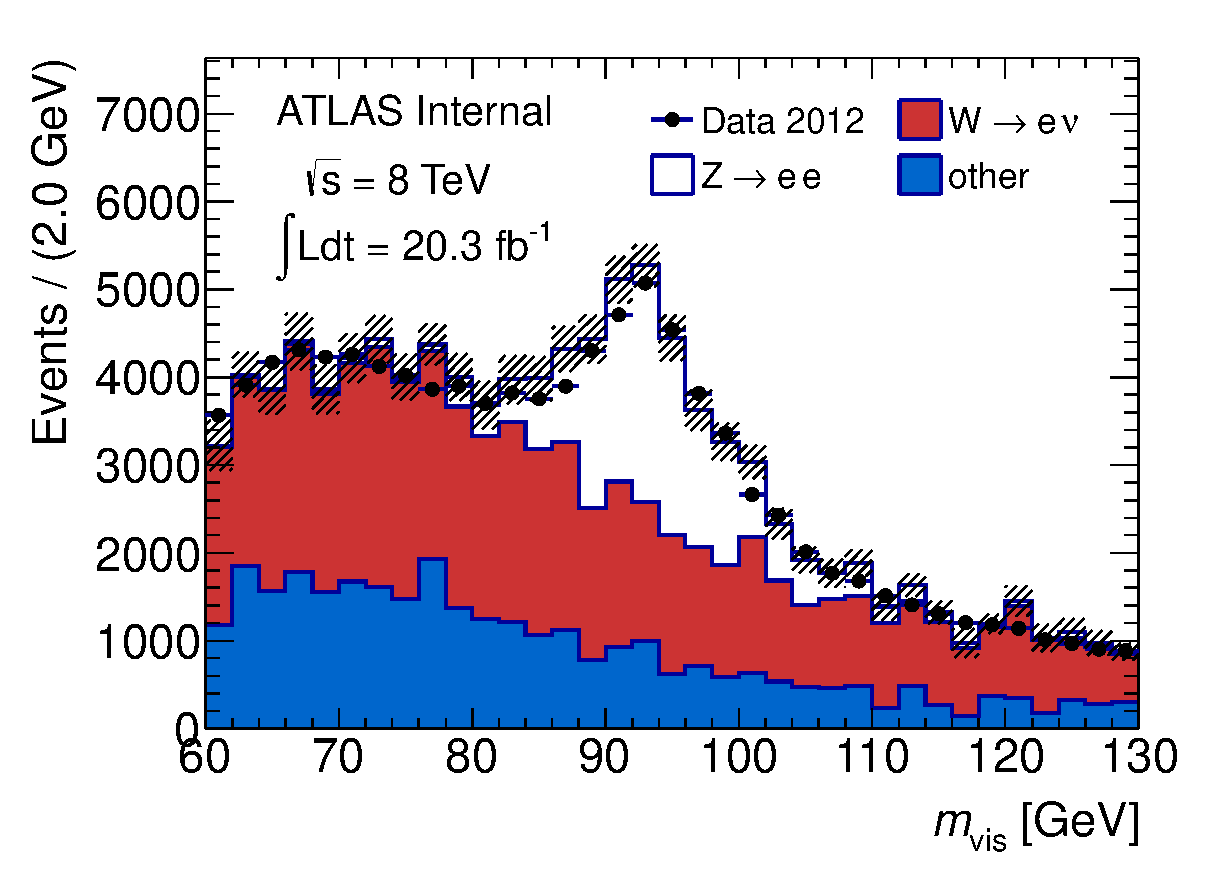
\includegraphics[width=0.48\textwidth]{figures/PERF-2013-06/eveto_mvis_mediumID_loosePPOLR_looseeveto}
  \caption{Variables.}
  \label{fig:taus-electronfakes2}
\end{figure}




\chapter[Evidence for decays of the Higgs boson to tau leptons][Evidence for decays of the Higgs boson to tau leptons]{Evidence for decays of the Higgs boson to tau leptons}
\include{tautau}

\chapter[Estimates for jets mis-identified as $\tau_\text{h}$][Estimates for jets mis-identified as $\tau_\text{h}$]{Estimates for jets mis-identified as $\tau_\text{h}$}
\include{fakes}

\chapter[Conclusions][Conclusions]{Conclusions}
\chapter[Conclusions][Conclusions]{Conclusions}
\label{chap:conclusion}

This thesis described evidence of Higgs boson decays to tau leptons with the ATLAS detector at the LHC, with special emphasis given to the VBF $\Htautaulh$ subset of the analysis. The theoretical context, LHC, and ATLAS experiment were briefly reviewed. The signature of tau leptons at ATLAS was described in detail.

The data in the $\Htautau$ analysis correspond to $20.3\ \ifb$ and $4.5\ \ifb$ of proton collisions at 8 TeV and 7 TeV, respectively. Strong evidence for $\Htautau$ is observed (expected) of a $4.5\sigma$ ($3.4\sigma$) deviation from the background-only hypothesis. The measured signal strength, normalized to the Standard Model expectation, is $1.4^{+0.4}_{-0.4}$, which is consistent with the Standard Model prediction. A limiting factor of the measurement is the size of the available dataset.

Future LHC data-taking campaigns will offer substantially more data and at a higher collision energy, though the harsh conditions present challenges for triggering on $\tauh$ and rejecting pileup jets mimicking the VBF signature. The VBF $\Htautaulh$ analysis projects to measure a signal strength uncertainty of 8\% with the addition of a high performance, high coverage forward tracker.


% \cref{chap:standardmodel} gives a description of the Standard Model of particle physics to provide theoretical context for searches for the Higgs boson. \cref{chap:lhcatlas} describes the LHC and the ATLAS detector, which are the experimental apparatuses used here. \cref{chap:taus} describes tau leptons and their experimental signatures at ATLAS.

% \cref{chap:strategy} describes the strategy for searching for $\Htautau$ at ATLAS. \cref{chap:backgrounds} reviews how physics processes relevant to the search are predicted, with special emphasis given to mis-identified $\tauh$. \cref{chap:results} gives the results of the searches. \cref{chap:prospects} concludes this thesis with a discussion of future prospects for $\Htautau$ analysis at ATLAS, both in the near- and long-term.




%%--------------------------------------------------------------------
%% appendix
%%--------------------------------------------------------------------
\appendix
\end{Spacing}

%%--------------------------------------------------------------------
%% bibliography
%%--------------------------------------------------------------------
\backmatter
\bibliographystyle{../style/atlasnote}
\bibliography{cross_sections,dark_matter,higgs,mc,measurements,performance,methods,detector,theory,lhc}

%%--------------------------------------------------------------------
\end{fmffile}
\end{document}
